
\chapter{Fundamentação Teórica}
\label{chap:fundam}
Neste capítulo será discutido na seção 2.1, algumas das ferramentas que já se propõe a realizar
a comparação de moléculas, assim como alguns dos algoritmos que podem ser utilizados na 
análise de similaridade molecular que serão apresentados na seção 2.3, sendo que parte desses 
algoritmos já estão adaptados em algumas das ferramentas a serem apresentadas.
Também será exposto na seção 2.2 algumas formas de representação de uma molécula em um 
ambiente computacional, e sua importância para escolha de qual método de comparação de 
moléculas deverá ser utilizado.
\newpage
\section{FERRAMENTAS PARA COMPUTAÇÃO DE SIMILARIDADE MOLECULAR}
\setcounter{equation}{1}
Devido a importância das ferramentas computacionais no processo de descobertas de fármacos, há diversos esforços dedicados ao desenvolvimento destas ferramentas, tornando-as cada vez mais eficientes e eficazes. Como resultado desses esforços, já se encontram disponíveis alguns sistemas computacionais que aplicam algoritmos de similaridade, realizam busca em bancos de dados, predição de propriedades físico-químicas e atividades biológicas, entre outras diversas funcionalidades importantes na pesquisa e desenvolvimento de fármacos. Esses softwares diferenciam-se de acordo com o custo de sua licença, funcionalidades implementadas, formatos de moléculas aceitos, representação computacional da molécula, método de computação de similaridade molecular, entre outros aspectos.

Uma das ferramentas populares entre pesquisadores na área de química medicinal é o ZINC. O sistema web ZINC é uma ferramenta livre que fornece para o usuário um banco de dados com mais de 21 milhões de estruturas catalogadas \cite{irwin2005zinc}. Além disso, o sistema armazena diversas informações  sobre cada molécula como : massa molecular, centros quirais, coeficiente de partição água-etanol calculado (cLogP). O ZINC armazena estruturas em formatos 2D, tal como o formato Simplified Molecular Input Line Entry System (SMILES), que são representações lineares utilizando uma sequência de caracteres para representação da estrutura molecular \cite{kumar2012}. Além do formato SMILES, o ZINC também aceita como formatos de entradas, Structure Data Format (SDF) e MOL2. O ZINC implementa rotinas para triagem virtual em sua base de dados utilizando os conceitos de similaridade molecular, permitindo ao pesquisador selecionar o grau de similaridade mínimo desejado, e retornando todas as moléculas em seu catálogo (banco de dados) com grau de similaridade igual ou superior ao selecionado pelo usuário \cite{irwin2005zinc}.

Outra ferramenta que pode ser utilizada para a comparação de similaridade entre moléculas é o software ANACONDA. Tal sistema realiza a computação da similaridade entre duas moléculas através da comparação de propriedades de suas respectivas superfícies moleculares utilizando projeção gnomônica . O emprego deste método permite	 a comparação de forma interativa de dois componentes, podendo sugerir modos de superposição entre as moléculas, e assim uma possível geração de um modelo famacofórico \cite{devillers1996}. Esta ferramenta apesar de apresentar bons resultados na comparação de similaridade molecular, não permite a comparação de mais de duas moléculas por consulta, e além disso também não fornece ao pesquisador nenhuma ferramenta para construção, ou manipulação de um banco de dados para catalogação das suas moléculas de estudo, exigindo assim um esforço para o mesmo catalogar suas moléculas de interesse, e realizar uma computação praticamente serial de similaridade entre moléculas que deseja-se estudar 

Utilizando uma abordagem para computação de similaridade molecular baseada na comparação de campos elestrostáticos e de campos de volume esférico, \cite{mestres1997mimic} descrevem um software denominado MIMIC, que implementa rotinas para realização de triagem virtual baseada na comparação de similaridade molecular. Este software permite ao pesquisador obter um índice de similaridade de alta precisão, pois consegue levar em consideração, além da estrutura da molécula, a contribuição de cada átomo na computação da similaridade molecular. Assim como descrito por \cite{devillers1996}, o MIMIC não realiza manipulação de banco de dados, por tanto necessita que o pesquisador insira as moléculas que deseja comparar na entrada do sistema de forma serial. Dessa maneira, para criar um banco de dados para catalogo de moléculas, o usuário necessita utilizar uma outra ferramenta para manipular bancos de dados, o que nem sempre é conveniente para um pesquisador que possua muitas moléculas para estudo, e que por muitas vezes não possui conhecimentos avançados de computação para fazer tal catalogação por conta própria.

Os esforços para implementação de ferramentas computacionais para cálculo de similaridade molecular não se restringem a programas de computador e/ou web sites. Alguns pesquisadores já tem desenvolvido bibliotecas multi-plataformas, capazes de interagir com várias linguagens de programação, e que implementam não somente rotinas para manipulação de moléculas em geral, mas também implementam algoritmos para computação de similaridade molecular. Nessa perspectiva, a Indigo Toolkit surge como uma das bibliotecas de acesso livre mais completas. Desenvolvida pela GGASoftware, e atualmente mantida pelo epam lifescience, Esta ferramenta é capaz de manipular os principais formatos disponíveis para representação de moléculas como: SMILES, SDF, Molfile, entre outros \cite{pavlov2011indigo}. O conjunto de ferramentas disponibilizado por essa biblioteca, permite ao usuário manipular moléculas, computar similaridade, buscar sub-estruturas e reações. A API indigo é capaz de utilizar diversos tipos de descritores moleculares, desde SMILES, até fingerprints (sequência de bits que representa presença ou ausência de uma determinada característica estrututral) e comparando moléculas através de diversas métricas como: coeficiente de Tanimoto, métrica euclidiana, e métrica de Tversky. Para sua utilização é necessário que esta biblioteca seja incorporada a um programa, que pode ser escrito em C/C++, java ou python. Esta biblioteca é utilizada na implementação do NatProDB, conforme será discutido posteriormente.

Utilizando uma abordagem de busca farmacofórica, O Pharmer é considerada uma ferramenta bastante robusta, e já tem sido utilizada até mesmo pelo Zinc no processo de triagem de moléculas similares em seu banco de dados \cite{koes2011pharmer}. O grande diferencial dessa ferramenta é a velocidade de processamento e computação de similaridade molecular em grandes bases de dados, chegando a ser uma ordem de magnitude mais rápido que as ferramentas computacionais já existentes \cite{koes2011pharmer}. O motivo para tal desempenho reside no fato de que em detrimento das demais ferramentas para triagem em bancos de dados moleculares através de modelos famacofóricos (que normalmente realizam a comparação serial de todas as moléculas de sua base de dados), o Pharmer utiliza uma estrutura de organização dados adaptada, denominada Pharmer KDB-tree data structure, e implementa um método de compração baseado em técnicas de computação visual: hashing geométrico e transformada generalizada de Hough. Através da utilização de tais tecnicas, o sistema não somente reduz o custo computacional para comparação de moléculas (grau de similaridade de modelos farmacofóricos), mas também reduz o tempo necessário para consulta no banco uma vez que a estrutura organizacional dos dados em sua base permite um direcionamento do sistema para alvos com maior probabilidade de serem similares.

Outra ferramenta pública que também implementa filtros baseados no conceito de similaridade molecular para triagem virtual de moléculas em bancos de dados (\textit{Virtual Screening})   é o Pubchem \cite{li2010pubchem}. Este sistema possui mais de 25 milhões de estruturas catalogadas em seu banco de dados, e é mantido pelo \textit{National Center for Biotechnology Information} (NCBI). O Pubchem é um dos sistemas bastantes difundidos na comunidade acadêmica devido ao fato de aceitar moléculas sob diversos formatos como (SDF, Mol, SMILES). Além disso, assim como o ZINC \cite{irwin2005zinc} por se tratar de uma fonte de pesquisa pública e de acesso via web, pesquisadores podem utilizar seus recursos computacionais independente de sua localização geográfica, auxiliando pesquisadores em diversos lugares no processo de desenvolvimento de ferramentas para modular processos biológicos e também na identificação de compostos com probabilidade de se tornarem medicamentos utilizados em tratamentos de doenças.   

\section{DESCRITORES MOLECULARES}
O descritor molecular pode ser considerado como o resultado da aplicação de procedimentos lógicos e matemáticos que transformam uma representação química codificada, em uma representação simbólica de uma molécula, em um formato padrão ou resultado de algum experimento padronizado, de forma a facilitar a manipulação dessas estruturas \cite{todeschini2008handbook}. Para o presente trabalho, o descritor molecular consiste no formato sobre o qual uma molécula é representada computacionalmente, e tal formato é importante para a computação de
similaridade, pois o descritor molecular é considerado um fator determinante da métrica a ser
aplicada para cálculo da similaridade estrutural. Nesta seção será apresentado alguns
descritores utilizados por sistemas que calculam similaridade entre moléculas\apud{todeschini2008handbook}{koes2011pharmer}.

\subsection{FingerPrints}
As Fingerprints podem ser consideradas como um descritor molecular complexo. Nesta forma representação computacional de uma molécula, todas as características e grupos funcionais presentes em um dado composto, são codificados em \textit{bitstreams} (Sequencia de bits 0 e 1) únicos para cada estrutura \cite{xue2000molecular}. Além dos grupos funcionais, e características inerentes a uma determinada molécula, as fringerprints também são capazes de armazenar em sua estrutura as distancias entre estruturas do composto, caminhos conexos dessa através de toda a estrutura molecular, ou diferentes tipos de farmacóforos de interesse do pesquisador \cite{todeschini2008handbook}.

Uma das vantagens na utilização de fingerprints na química computacional, é a capacidade de armazenamento de características intrísecas de um composto em um formato de relativamente fácil manipulação por sistemas computacionais. Por exemplo, dentre os modelos de fingerprints mais utilizados na química-computacional, podemos citar a Daylight fingerprint, que utiliza em torno de 2048 bits para armazenamento de propriedades, características, e distâncias moleculares de um único composto, sendo que para esse tipo de descritor não ocorre uma relação direta entre um bit e um determinado grupo funcional/característica (como em modelos de figerprints mais simples), na verdade determinadas caracteristicas, distancias, e/ou propriedades podem ser mapeadas através de algorítmos de \textit{Hashing} para fornecer assim padões de bits cada vez mais específicos, permitindo maior fidelidade na representação das propriedades de uma molécula em um sistema computacional \cite{xue2000molecular}.

Outra importante vantagem da utilização de figerprints para representação computacional de uma molécula reside na simplicidade de aplicação de métodos e métricas para comparacação moléculas baseado no conceito de similaridade molecular \cite{xue2000molecular}. Nesta perspectiva, devido as características intrísicas  desse descritor molecular, o processo de triagem virtual em um banco de dados molecular, pode ser realizado através da geração de fingerprints para cada uma das moléculas do banco e da molécula de consulta, e da aplicação de métricas de similaridade molecular de relativamente fácil implementação em sistemas computacionais como: Coeficiente de Tanimoto, Coeficiente de Tversky, Dice entre outras, que basicamente obtem um determinado coeficiente de similaridade entre duas estruturas moleculares através da realização de um cálculo estatístico que leva em consideração as estruturas e caracteristicas compartilhadas e as singulares das moléculas comparadas. No sistema NatProDB, as fingerprints possuem um papel fundamental no processo de triagem de moleculas de seu banco de dados, uma vez que tal descritor é utilizado para comparação de moléculas conforme será descrito mais aprofundadamente no próximo capítulo.  
     

\subsection{Descritores Farmacofóricos 3D}
Os descritores farmacofóricos tridimensionais quantificam propriedades e as distâncias entre  farmacóforos biológicos importantes para a interação entre o ligante e receptor  \cite{bajorath2004chemoinformatics}. Dentre essas propriedades de interesse de pesquisadores podemos citar: grupos funcionais ou características chaves em determinada orientação, doadores/receptores de ligações de hidrogênio, partes de uma molécula, entre outras. Normalmente, um descritor farmacofórico 3D são compostos basicamente por 3 ou 4 características, e de 3 a 6 distancias entre elas. 
Quando a conformação biológica entre o ligante e receptor é conhecida, é possível identificar     
que características/grupos funcionais são cruciais para ocorrencia dessa ligação. Caso contrário, através de técnicas de triagem virtual (\textit{virtual screening}) pesquisadores podem identificar moléculas que contenham esses grupos funcionais/caracteristicas, ou até mesmo projetar um descritor farmacofórico 3D \cite{bajorath2004chemoinformatics}. 
A aplicação de ferramentas computacionais na comparação de moléculas representadas como descritores farmacofóricos 3D pode ser realizada através do conceito de similaridade molecular aplicando uma transformação nesse descritor em uma \textit{figerprint} (Sequência de bits única para uma molécula), onde bits definidos como '1' simbolizam a presença de uma determinada caracteristica ou grupo funcional, e bits definidos como '0' a ausência de tal estrutura na molécula. Sendo assim, ferramentas computacionais podem calcular a similaridade entre duas moléculas gerando figerprints para cada um dos descritores farmacofóricos 3D e aplicando alguma das métricas já conhecidas para calculo de similaridade entre figerprints, como por exemplo coeficiente de Tanimoto, e coeficiente de Tversky, ambos serão descritos com maiores detalhes em sessões posteriores.          

\subsection{SMILES (Simplified Molecular-Input Line-Entry System)}
     
O SMILES surgiu como descritor molecular para resolver não somente o problema de 
armazenamento de estruturas moleculares em um computador, mas também facilitar a 
manipulação dessas estruturas moleculares por softwares, e também facilitar buscas por 
estruturas moleculares em base de dados na internet internet \cite{kumar2012}. Ainda segundo \cite{kumar2012} é demonstrado que pode-se considerar o SMILE como uma linguagem que permite ao pesquisador representar uma molécula através de uma notação linear padronizada, que muito 
se assemelha à notação utilizada comumente na literatura.

Em uma representação de molécula em formato de SMILES cada átomo é representado por seu símbolo atômico, onde os hidrogênios são omitidos \cite{anderson1987smiles}. Os átomos vizinhos, são representados próximos entre si, e em caso de ligação dupla ou tripla, entre os átomos unidos por tais ligações aparecerão respectivamente os símbolos = e \#. É importante salientar também que ramificações são representadas por parêntesis, e os anéis aromáticos pela alocação de dígitos entre os dois átomos que fecham o anel. A figura 2 exemplifica a conversão de uma estrutura tridimensional em uma notação SMILE, e como tal representação se assemelha a forma como a literatura

\begin{figure}[!htb]
	\centering
	\caption[Exemplo de Molécula representada em SMILE]{Exemplo da representação de uma estrutura 3D em SMILES.}
	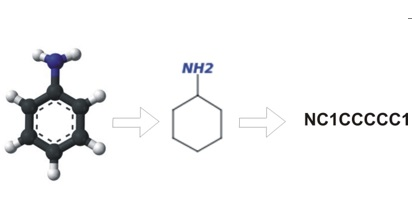
\includegraphics[width=0.5\textwidth]{SMILE.jpg} % <- formatos PNG, JPG e PDF
	\fonte{Autor\nocite{abnTeX2009}}
	\label{fig:dummy}
\end{figure}

O formato do SMILE gerado para a molécula não é necessariamente único, existem
outras representações possíveis, dependendo da estratégia de notação adotada pelo 
pesquisador. Dessa forma é muito comum, para facilitar a busca em bancos de dados, a 
utilização de um formato SMILE canônico, ou seja, que padroniza qualquer SMILE para um 
formato único, o que simplifica a manipulação de qualquer molécula, sem aumentar a 
complexidade dessa operação para o pesquisador (KUMAR, 2012).

Este descritor molecular, além de necessitar de recursos computacionais relativamente 
baixos para representação de uma molécula, devido sua estrutura, é 
bastante utilizado no desenvolvimento de fármacos, principalmente nas atividades que 
envolvem a busca de estruturas similares com uma desejada atividade biológica, pois por ser 
um descritor molecular linear, ele permite a simplificação de uma comparação de moléculas 
realizadas por exemplo em uma forma tridimensional, em uma comparação linear de cadeias 
de caracteres, de mais fácil manipulação em um computador. 

\section{Algorítmos e Métricas para Computação de Similaridade Molecular}

A busca por similaridade molecular é um ponto importante no projeto de um
fármaco pois tal conceito é um dos norteadores para triagem virtual de moléculas de interesse em bancos de dados. Os algorítmos e métricas utilizados na comparação de moléculas baseados no conceito de similaridade são dependentes do descritor molecular utilizado, logo a orientação do método de comparação selecionado deve ser direcionada pela escolha da melhor forma para representar a molécula computacionalmente (TODESCHINI; CONSONNI, 2000). Tal afirmação permite inferir que uma escolha não-adequada de descritor molecular para aplicação de um algoritmo pode inviabilizar a aplicação do mesmo, assim como retornar resultados indesejados, ou não fidedignos com a literatura, prejudicando assim a pesquisa.

\subsection{Coeficiente de Tanimoto}

Existem diversas métricas utilizadas para determinação de similaridade entre duas
moléculas, em geral elas geram um score indicando o grau de similaridade dos compostos comparados. Algumas dessas métricas utilizam distancias euclidianas para determinar esse 
score, como no caso das métricas de Hamming, e Euclidiana. É comum também a utilização 
de coeficientes de associação tais como: Tanimoto, Dice, e coeficientes de cossenos.

O coeficiente de Tanimoto realiza a comparação de moléculas através de uma simples contagem de características compartilhadas (grupos funcionais, propriedades, etc) entre as moléculas submetidas à comparação. Essa contagem gera um determinado valor entre 0 e 1 que indica o grau de similaridade entre as estruturas verificadas \cite{Dogra2007}.

O coeficiente de Tanimoto pode ser utilizado na comparação de descritores moleculares 2D. Nessa perspectiva, este coeficiente se mostra bastante efetivo na comparação de similaridade entre moléculas representadas computacionalmente como \textit{fingerprints}, pois devido a estrutura desse descritor molécular, a comparação de similaridade pode ser realizada através de op
erações booleanas em cadeias binárias para contagem do número de caracteristicas em comum entre cada par de fingerprints \cite{willett2003similarity}. Dessa maneira, a aplicação do coeficiente de Tanimoto para medir similaridade entre duas fingerprints A e B pode ser realizada tomando $N_{A}$ como o número de caracteríticas presentes em A (bits iguais a 1 em A), $N_{B}$ como o número de caracteríticas presentes em B (bits iguais a 1 em B), $N_{AB}$ como o número de caracteríticas compartilhadas por A e B (bits iguais a 1 em A e B), e finalmente o coeficiente de Tanimoto $T_{C}$ pode ser obtido aplicando a equação\eqref{eq:Tanimoto} 

\begin{equation}
T_{C} =\frac{N_{AB}}{N_{A}+N_{B} - N_{AB}}
\label{eq:Tanimoto}
\end{equation}

Nota-se em na equação (\ref{eq:Tanimoto}), que somente são considerados na computação do 
coeficiente de Tanimoto a presença das estruturas (características), a ausência não interfere 
neste processo, o que otimiza a comparação dessas estrutura \cite{Dogra2007}.

\subsubsection{Aplicação do Coeficiente de Tanimoto na Comparação de Fingerprints} 

Seguindo a descrição do coeficiente de Tanimoto apresentada por \cite{Dogra2007}, o trabalho de \cite{machao2011gpu} descreve a utilização dessa métrica para comparação de fingerprints. Em resumo, cada fingerprint presente no banco de dados do autor é representada como vetores de bits com 992 posições, ou seja, para cada molécula são 
verificadas a presença ou ausência de 992 estruturas (características) \cite{Dogra2007}. 

Após verificada essa presença ou ausência dessas estruturas nas moléculas, ou seja gerada a 
fingerprint, é aplicada a equação (\ref{eq:Tanimoto}) sobre as moléculas que se deseja comparar. Assim é obtido o score de similaridade entre as estruturas, e verifica-se se há similaridade ou não entre as moléculas submetidas, conforme podemos observar na  figura (\ref{fig:comparafingerprint}).
\begin{figure}[!htb]
	\centering
	\caption[Cálculo do Coeficiente de Tanimoto sobre duas Fingerprints]{Aplicação do coeficiente de Tanimoto para Computar Similaridade entre Fingerprints.}
	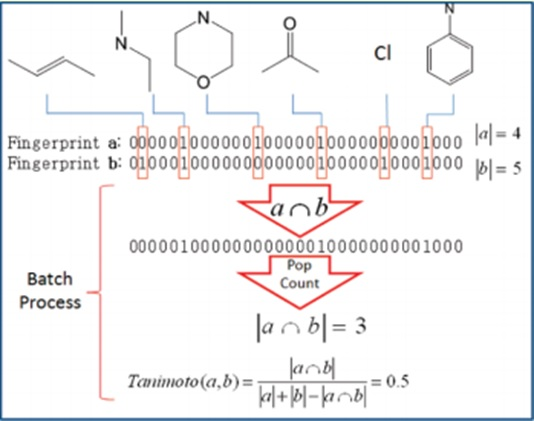
\includegraphics[width=0.5\textwidth]{comparacao_fingerprints.jpg} % <- formatos PNG, JPG e PDF
	\fonte{\cite{machao2011gpu}}
	\label{fig:comparafingerprint}
\end{figure}

Apesar foco central do trabalho apresentado por \cite{machao2011gpu}, não ser a comparação de similaridade molecular, mas sim a paralelização do processo de comparação de similaridade entre bancos de dados moleculares, a figura \ref{fig:comparafingerprint} extraída de sua 
obra, ilustra o procedimento de comparação entre fingerprints, exemplificando desde a 
contagem de estruturas (características) na fingerprint \textit{a} , e na fingerprint \textit{b}, assim como a intersecção entre as características de ambas estruturas ($a\bigcap b$), e por fim a computação do coeficiente de Tanimoto. De acordo com \cite{Dogra2007}, o resultado do coeficiente de Tanimoto (0,5) obtido na figura (\ref{fig:comparafingerprint})  indica baixa similaridade entre as moléculas a e b.

\subsection{Lingo}

O método proposto por \cite{vidal2005lingo} denominado LINGO realiza a computação da similaridade entre moléculas através da conversão dos SMILES de cada molécula (descritor molecular) em um conjunto de substrings sobrepostas de tamanho definido (o autor sugere tamanho 4 para melhores resultados). Desta forma evita-se a manipulação de estruturas tridimensionais, e de grafos, que são mais complexos para se tratar computacionalmente.

Para gerar cada subestrutura do conjunto de substrings a ser utilizado, é necessário a
realização de uma canonização do SMILE, onde converte-se o SMILE de cada molécula para 
uma forma padronizada, conforme já exposto anteriormente. Uma vez canonizadas, as 
SMILES de cada molécula são quebradas em n-(q-1) subestruturas, onde n é o número de 
caracteres do SMILE, e q é o tamanho definido para cada subestrutura. Os conjuntos de 
subestruturas quebradas a partir dos SMILES das moléculas a serem comparadas, são 
agrupados em vetores para aplicação da métrica de similaridade \cite{vidal2005lingo}.

Para computar a similaridade entre os dois vetores (que passaram a representar as 
moléculas), é utilizado o coeficiente de Tanimoto, mas em um formato modificado como podemos verificar na equação \eqref{eq:Modificado}

\begin{equation}
T_{C} =\frac{\sum\limits_{i=1}^{l}1-\frac{|N_{A,i}-N_{B,i}|}{N_{A,i}+N_{B,i}}}{l}
\label{eq:Modificado}
\end{equation}

Observando a equação \eqref{eq:Modificado} verifica-se que $N_{A,i}$ corresponde ao número de ocorrências da i-ésima subestrutura na molécula A (vetor de subestruturas de A), e $N_{B,i}$ o número de 
ocorrências da i-ésima subestrutura na molécula B (vetor de subestruturas de B), e l indica o 
comprimento de um vetor união ($A\bigcup B$). Dessa forma devido ao somatório presente no 
numerador, quanto mais idênticas as frequência de aparições de cada subestrutura em ambas 
moléculas, mais alto será o coeficiente de Tanimoto entre as mesmas, indicando assim uma 
maior similaridade.

\subsection{Localized Co-occurrence Model (LCM)}
Este algoritmo é utilizado para computação de similaridade sobre moléculas
representadas por coordenadas tridimensionais. Segundo \cite{huang2008localized} cada átomo é representado por uma tripla (x,y,z), que informa suas respectivas coordenadas em um espaço tridimensional, e assim para cada átomo, são buscados seus três outros átomos mais próximos, formando um tetraedro denominado Unit Structure, este procedimento é realizado para todos os átomos de uma molécula.

Para cada Unit Structure é calculado o seu volume, e assim então para cada molécula 
será obtido um conjunto de Unit Structures que terá associado as mesmas um valor de 
volume, e então o algoritmo utilizará o menor volume obtido, e o maior volume encontrado 
para definir os limites de um intervalo de volumes para esta molécula. Além disso são 
definidos um conjunto de estados que será associado ao intervalo de volumes, dessa forma o 
intervalo de volumes será particionado de acordo com a quantidade de estados definidos para 
a molécula. Cada Unit Structure recebe um valor de estado correspondente à partição de 
volume que a mesma pertence.

Após definido o estado de cada Unit Structure, para cada par de UnitsStructures o
algoritmo faz uma conexão entre elas caso o centro de massa entre as mesmas seja menor que 
um valor definido, este procedimento é realizado para todos os possíveis pares que podem ser 
formados dentro de um conjunto de Unit Structures. Uma vez formadas todas as conexões 
possíveis, o algoritmo verifica a co-ocorrência das relações das Unit Structuresem relação aos seus valores de estado \cite{huang2008localized}.

Por fim este algoritmo computa a probabilidade de co-ocorrência para cada
combinação de pares de estados, gerando para cada molécula um LCM. A similaridade entre 
duas moléculas é determinada pela comparação dos LCM deLCM de cada uma delas, e 
verificando o grau de semelhança entre as representações das moléculas em forma de LCM, 
quanto mais parecidos os LCMs maior a similaridade entre as moléculas, em contrapartida 
quanto menor a semelhança entre os mesmos, menor a similaridade entre as moléculas.





Neste capítulo foram apresentadas algumas das ferramentas utilizadas por pesquisadores
para comparação de moléculas com determinados graus de similaridade. Foi apresentado 
também algumas das principais formas de representação de uma molécula 
computacionalmente (de agora em diante denominada descritores moleculares), e sua 
influência na escolha do algoritmo para computação da similaridade molecular. Além disso 
foi discutido alguns dos algoritmos e métricas possíveis de utilização para realizar tal atividade,contando com uma pequena descrição prévia do selecionado para utilização neste trabalho.No próximo capítulo será discutida as ferramentas utilizadas na adaptação do algoritmo selecionado, bem como a metodologia aplicada para avaliar algoritmo adaptado 
ao sistema NatProDB.


